\documentclass{article}
\usepackage[left=0.5in,top=0.5in,right=0.5in,bottom=0.5in]{geometry}
\usepackage[english]{babel}
\usepackage[utf8]{inputenc}
\usepackage[table]{xcolor}
\usepackage{graphicx}
\usepackage{soul}
\usepackage{
  changepage,
  threeparttable
}
\usepackage{
  booktabs,
  multirow
}
\usepackage{
  amssymb,
  amsmath,
  amsthm,
  latexsym
}
\graphicspath{{./images/}}
\def\R#1#2{\(R_{\text{\tiny#1,\tiny#2}}(\Omega)\)}
\def\RTH#1#2{R_{\text{\tiny#1,\tiny#2}} (\Omega)}
\def\RP#1{R_{\text{\tiny#1}}}
\def\RS#1{R_{\text{\tiny#1}}}
\def\OHMs{~\Omega}
\def\OHM{~\(\Omega \)}
\title{Lab 4: Resistor Networks}
\author{Philip Kim}
\date{\today}
\begin{document}
\maketitle
\begin{table}[!htp]\centering
  \subsection*{Part 1}
  \begin{tabular}{|c|c|c|c|c|c|c|}\hline
  \multicolumn{6}{|c|}{\textbf{Table 1: Parallel networks}} \\\hline
  \R{1}{th} & \R{1}{exp} & \R{2}{th} & \R{2}{exp} & \R{P}{th} & \R{P}{exp} \\\hline
  1k & 0.999 & 2k & 1.990k & 0.6651 & 0.666 \\\hline
  1k & 0.999 & 510 & 0.511 & 0.3381 & 0.357 \\\hline
  1k & 0.999 & 3.3k & 3.290k & 0.7663 & 0.770 \\\hline
  10k & 9.970k & 5.1k & 5.070k & 3.3609k & 3.360k \\\hline
  10k & 9.970k & 20k & 19.940k & 6.6467k & 6.620k \\\hline
  10k & 9.970k & 47k & 47.400k & 8.2374k & 8.200k \\\hline
  \end{tabular}
  \begin{center}
    \subsection*{Picture: \R{1}{exp},~\R{2}{exp},~\R{P}{exp}}
    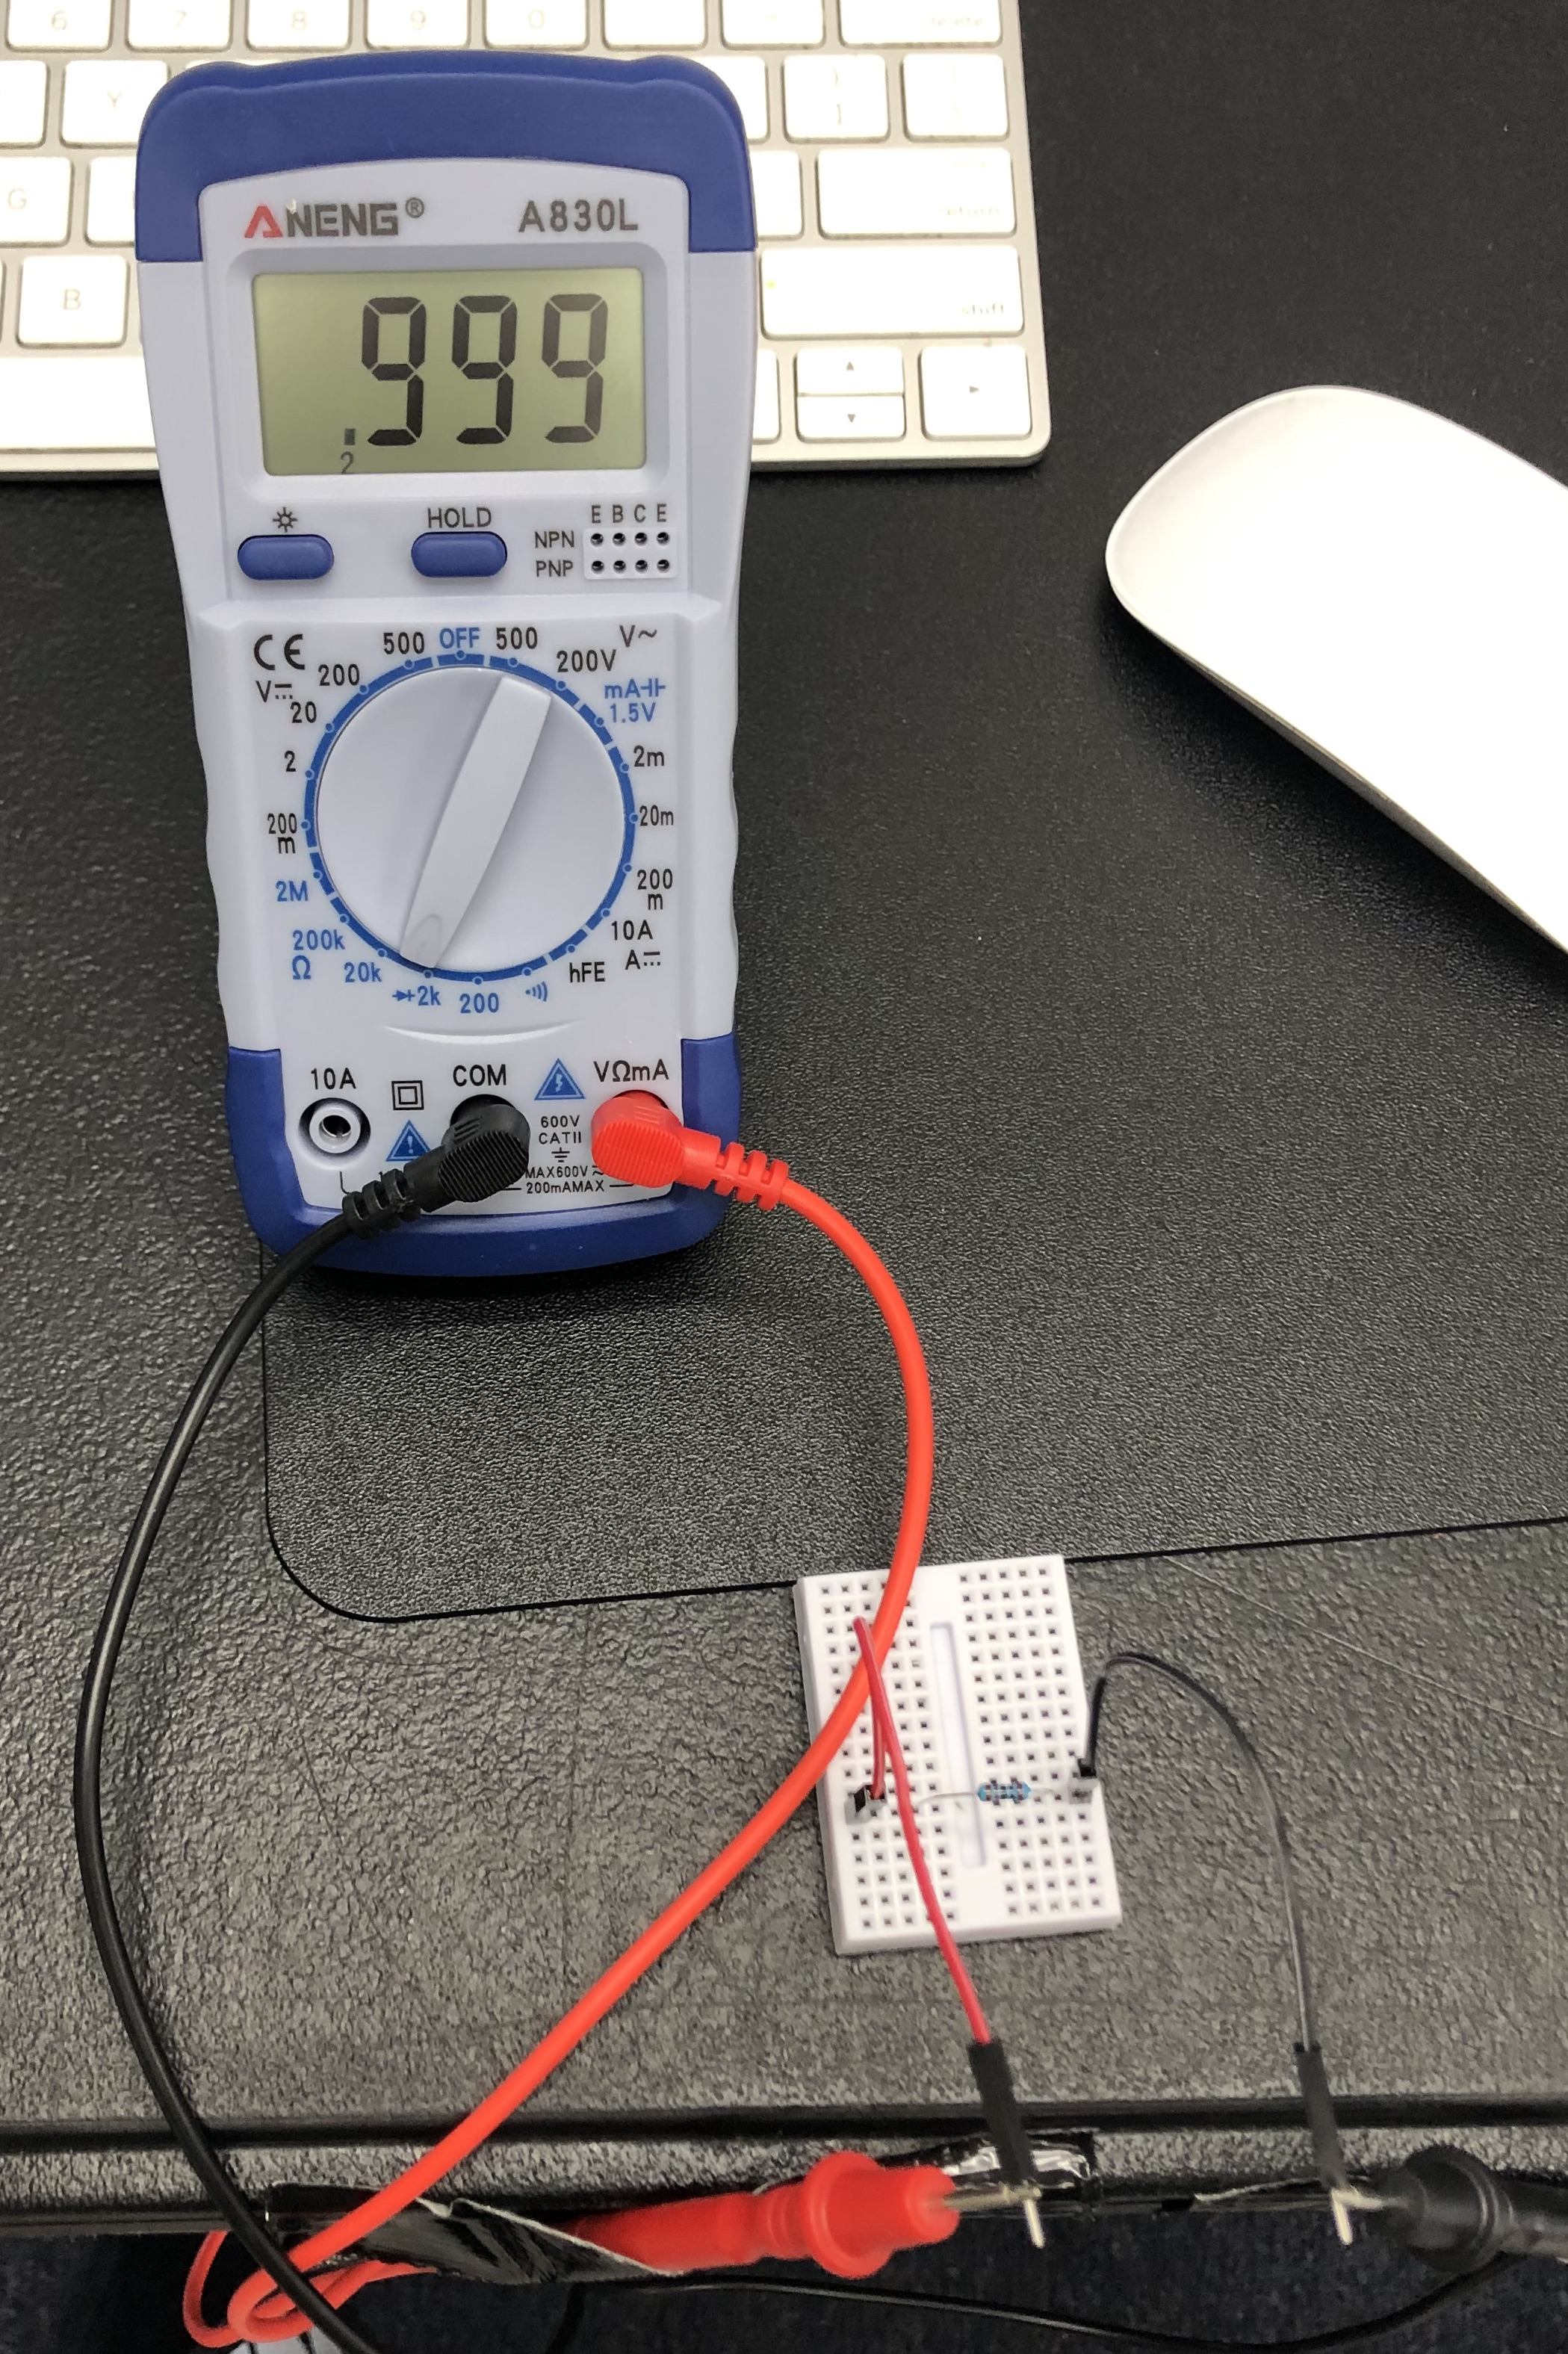
\includegraphics[scale=0.079,height=4.5cm]{R1.jpeg}
    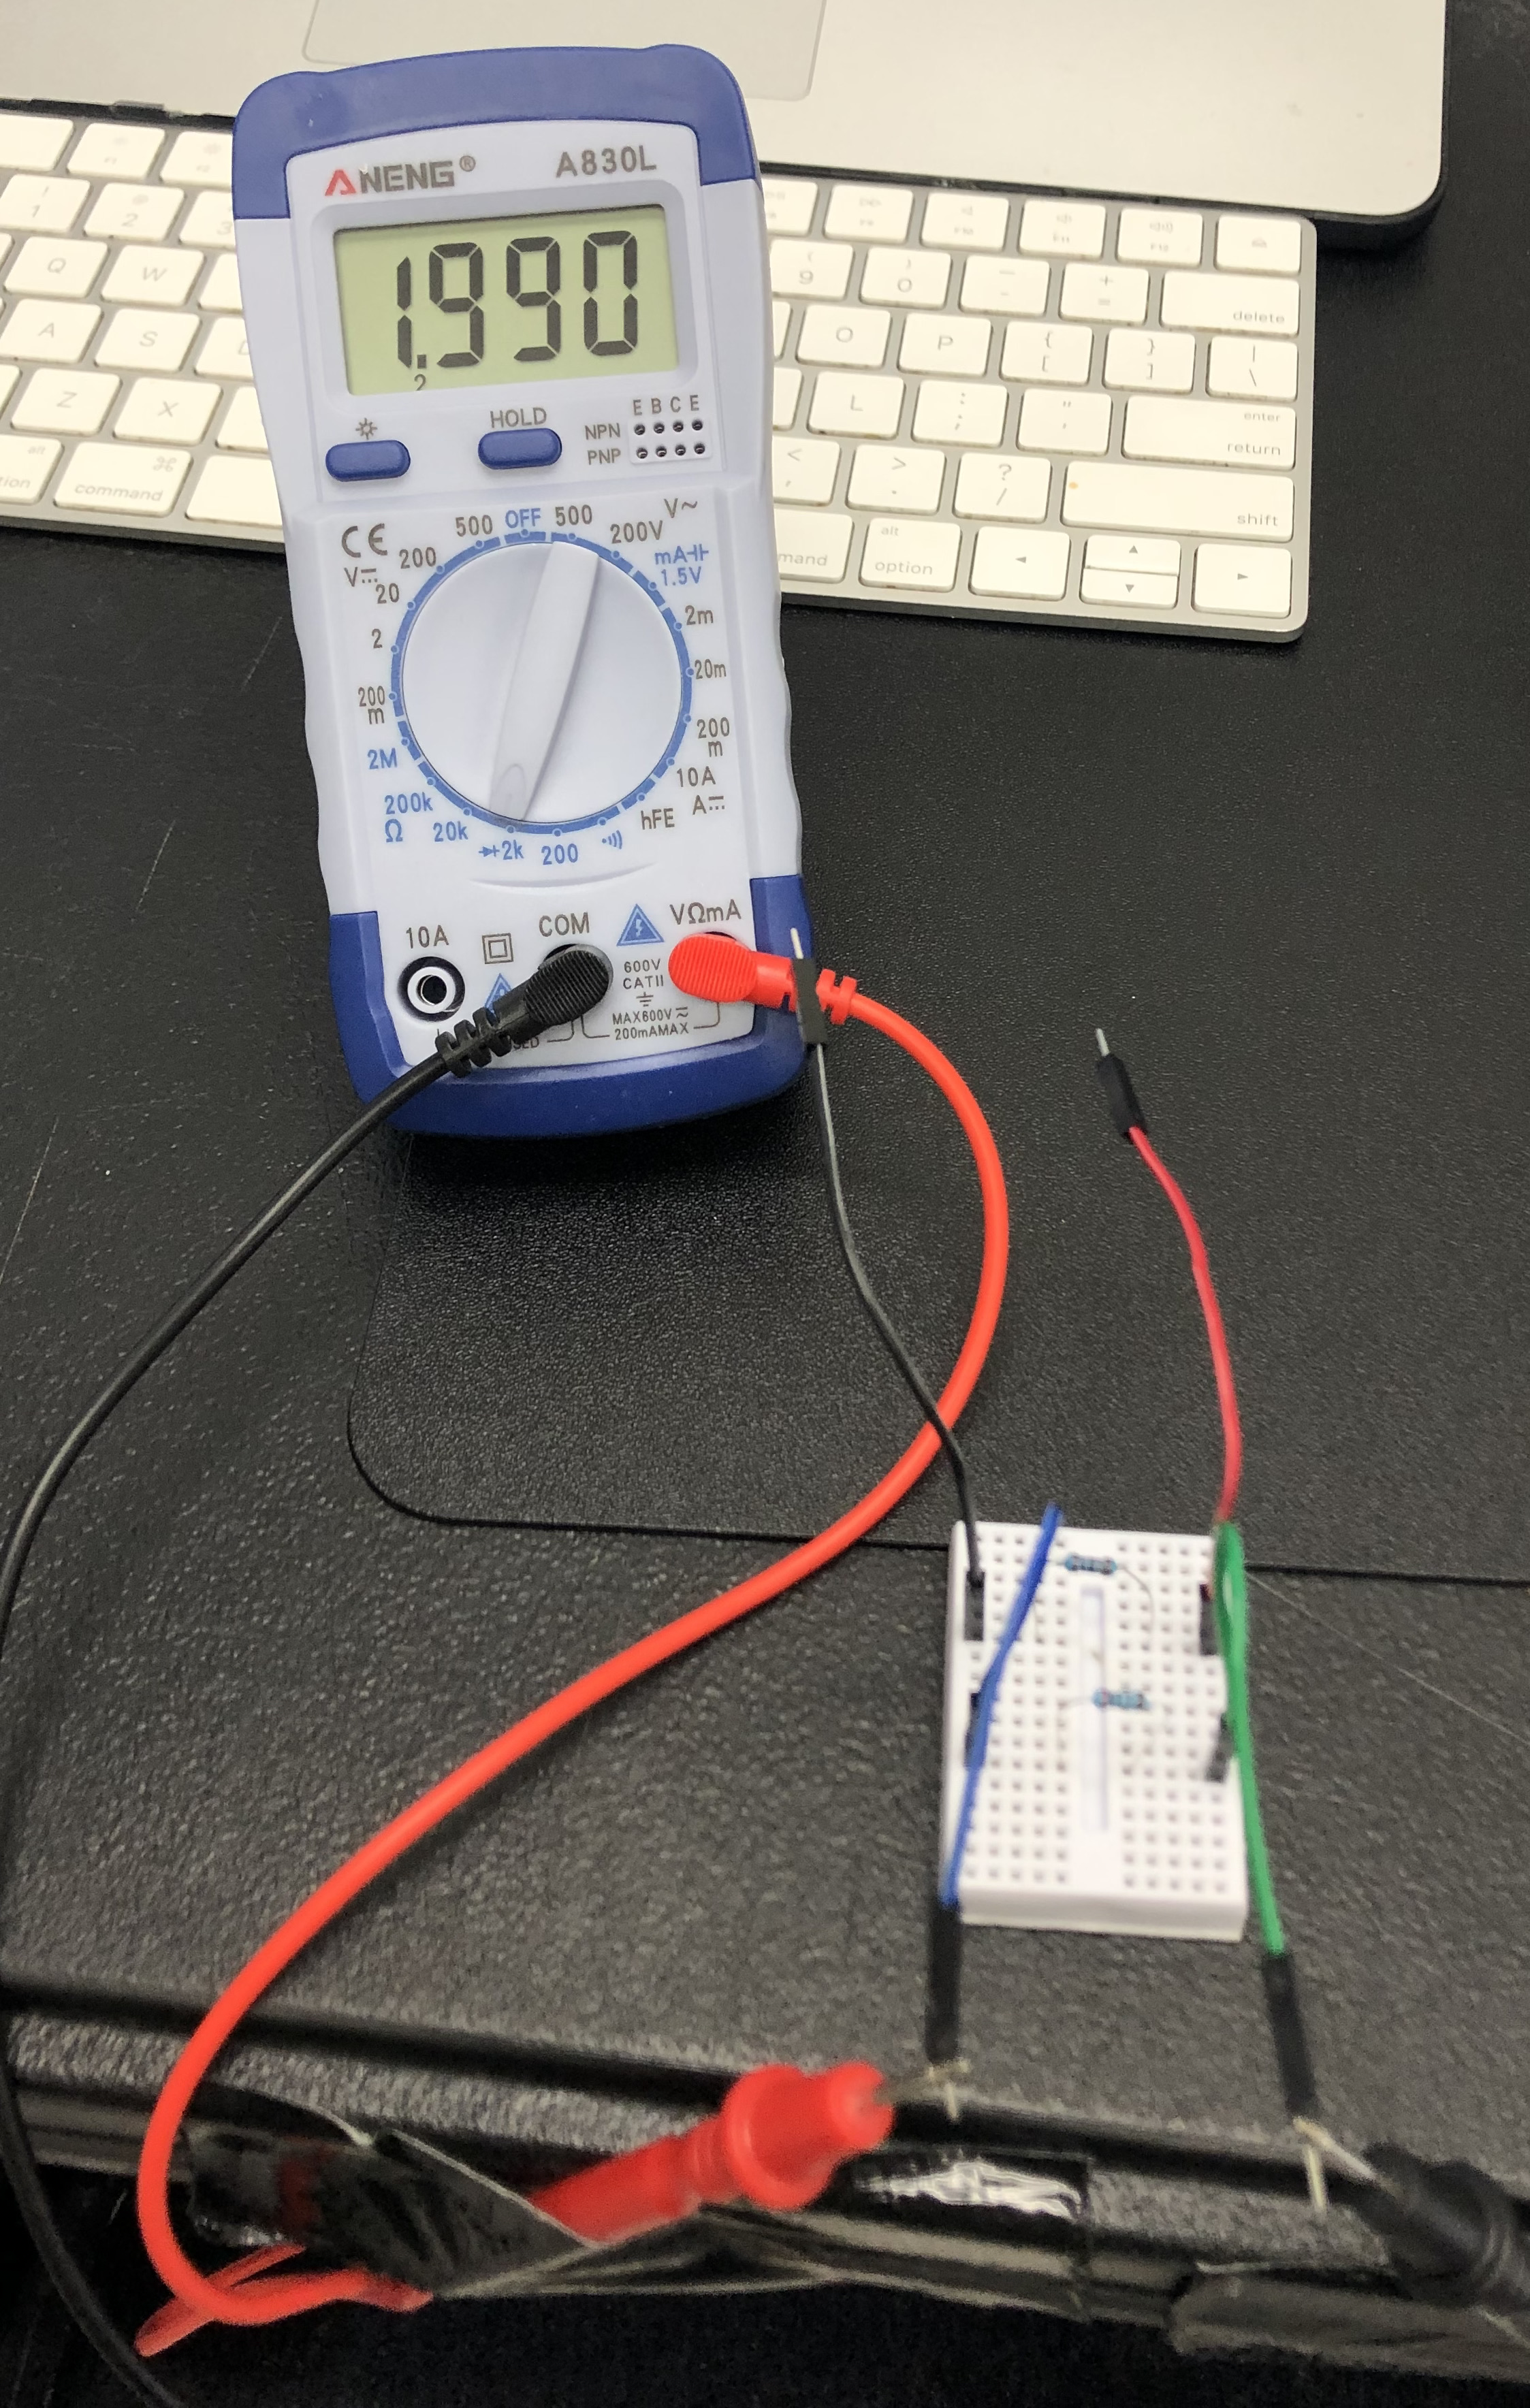
\includegraphics[scale=0.070,height=4.5cm]{R2.jpeg}
    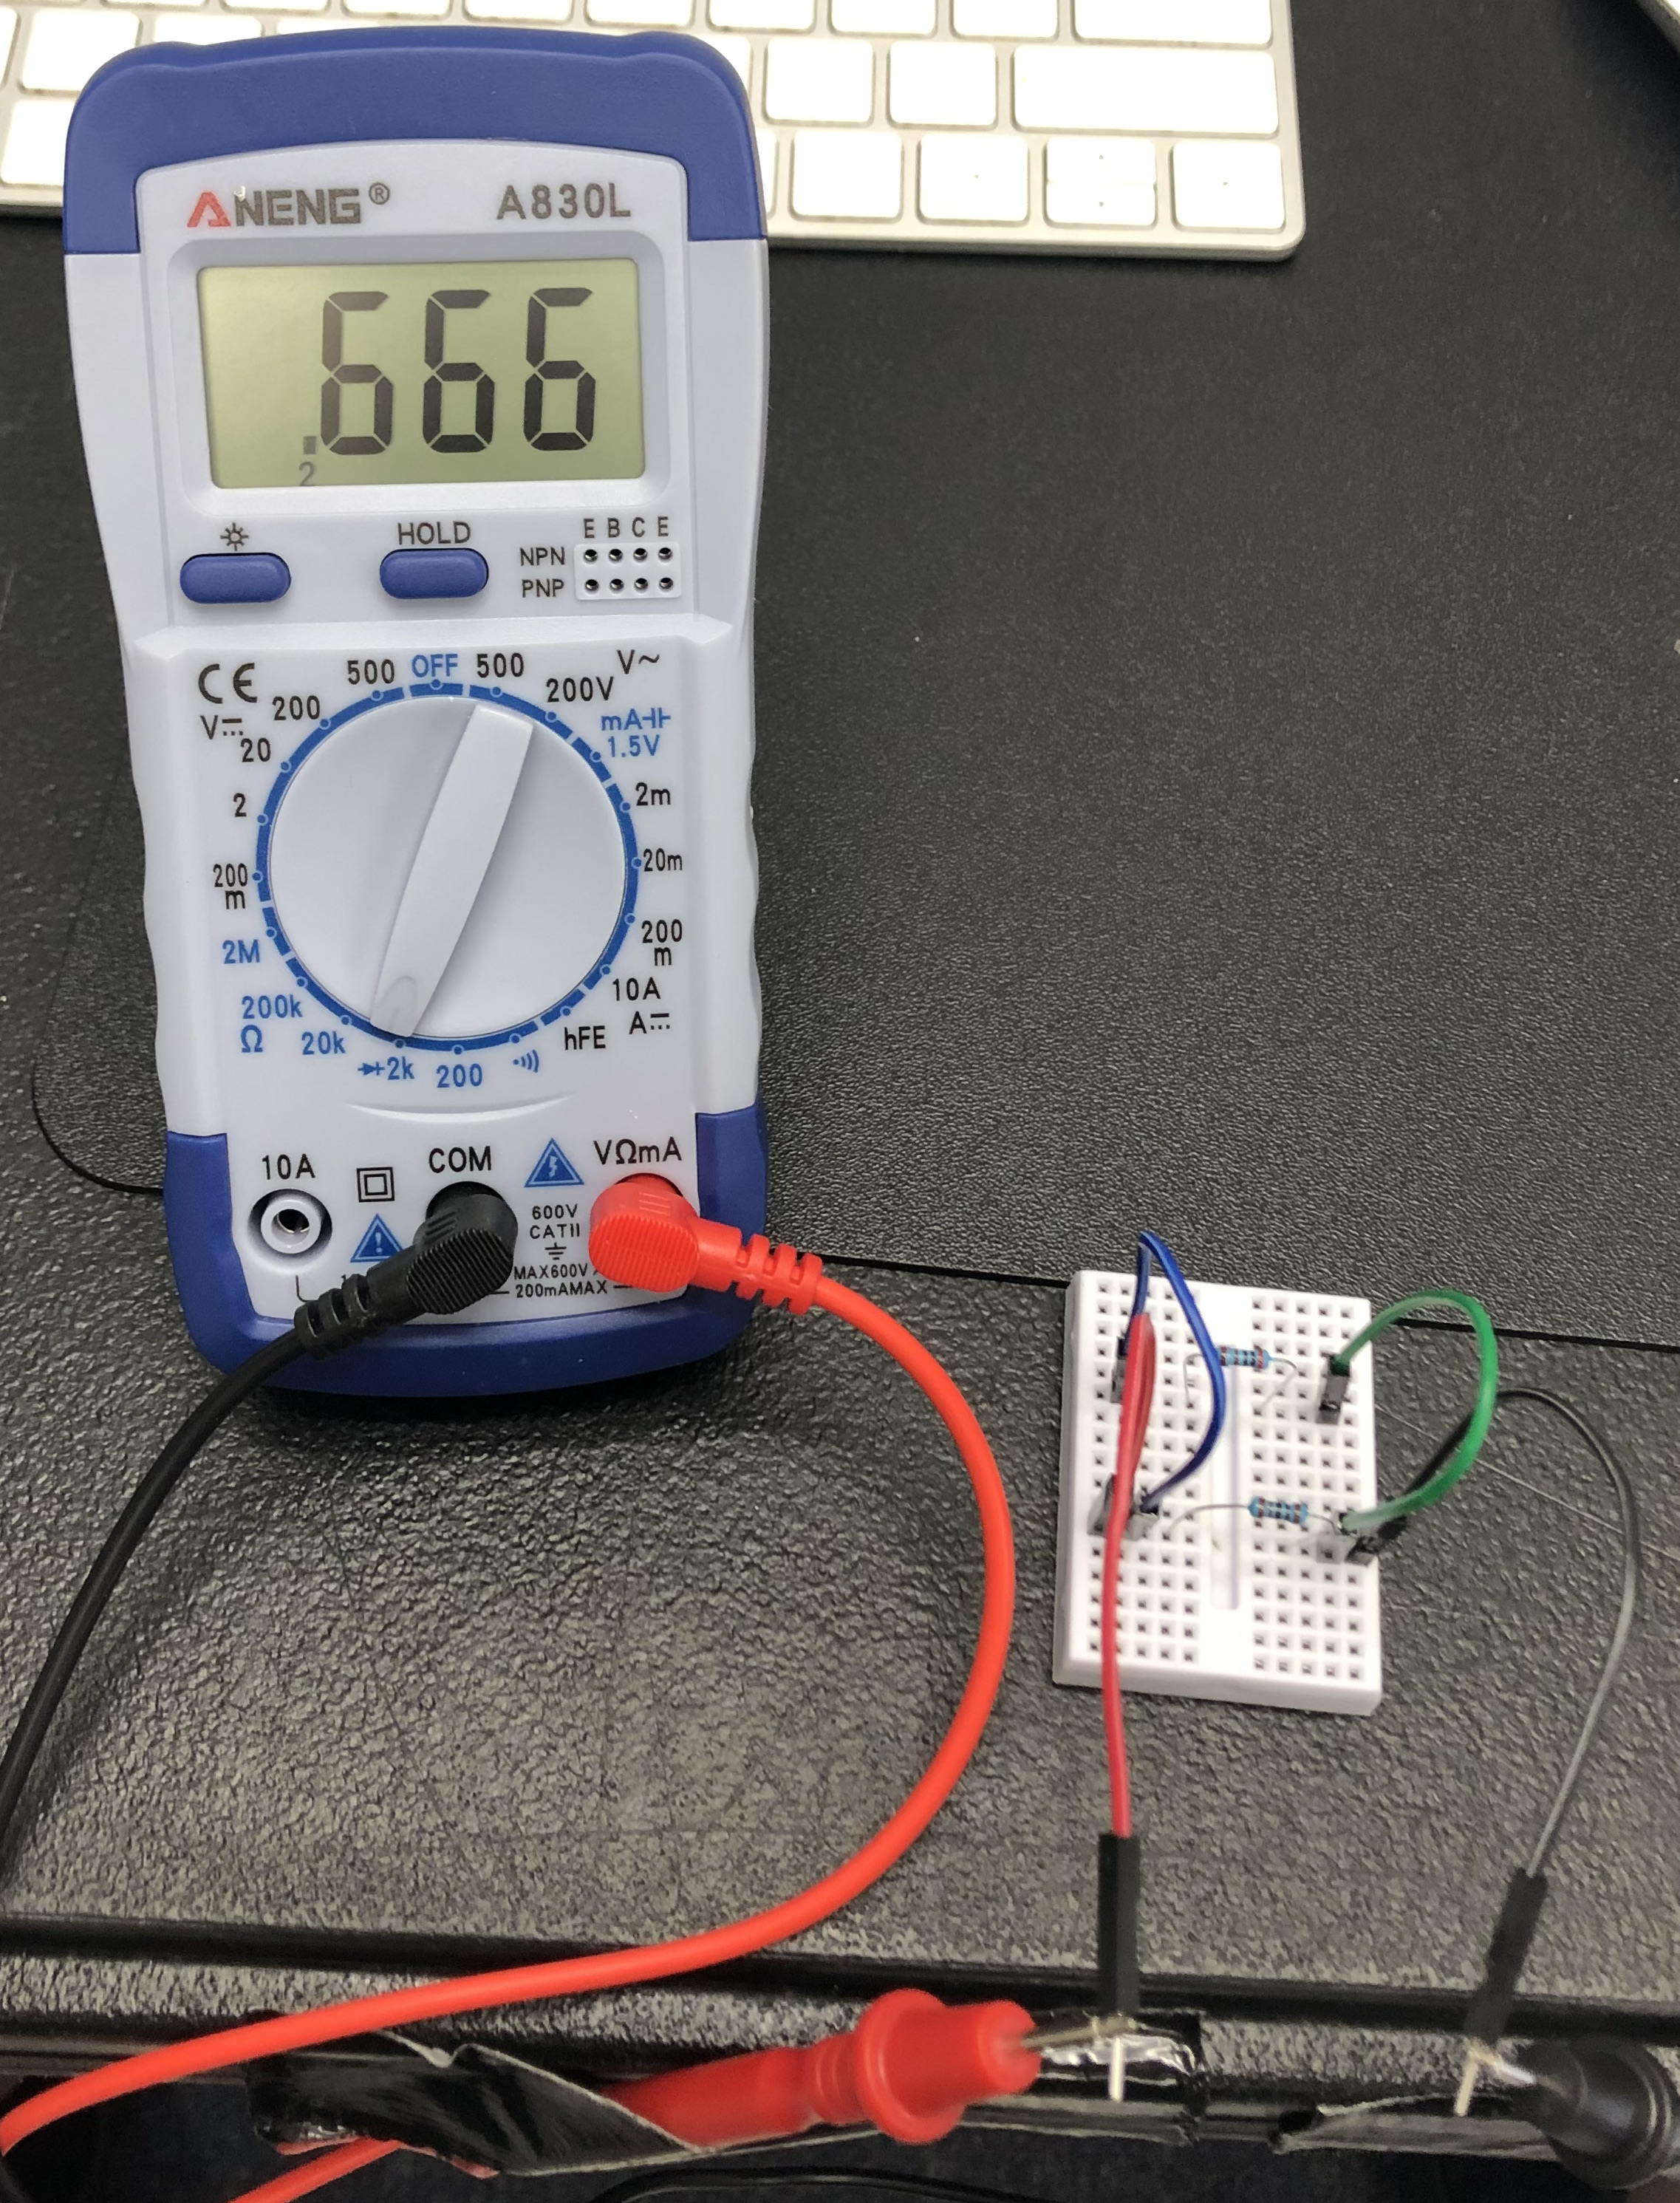
\includegraphics[scale=0.083,height=4.5cm]{RP.jpeg}
    \subsection*{Graph 1}
    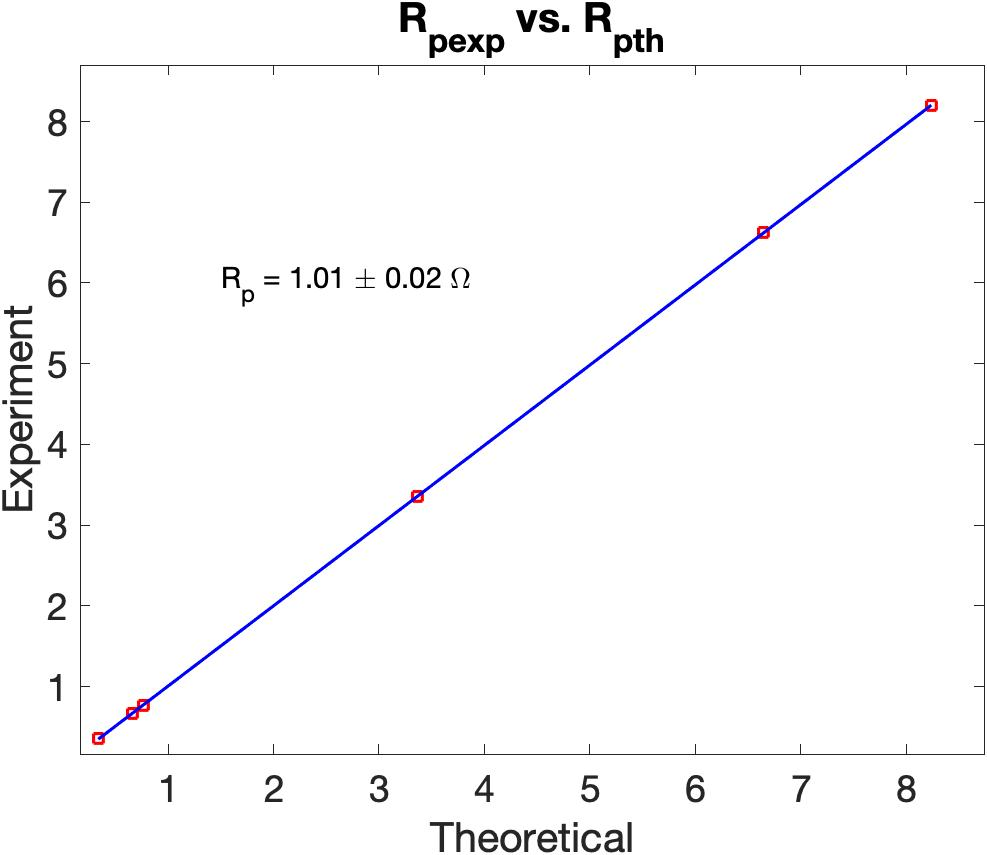
\includegraphics[scale=0.18]{RP_graph.jpeg}
    \subsection*{Discussion 1}
    \begin{enumerate}
      \item Discuss how well the experimental values of the parallel networks followed the theoretically expected value and quantify that relation.
      \begin{itemize}
        \item
      \end{itemize}
    \end{enumerate}
  \end{center}
\end{table}
\newpage
\begin{table}[!htp]\centering
  \subsection*{Part 2}
  \begin{tabular}{|c|c|c|c|c|c|c|}\hline
  \multicolumn{6}{|c|}{\textbf{Table 2: Parallel networks}} \\\hline
  \R{1}{th} & \R{1}{exp} & \R{2}{th} & \R{2}{exp} & \R{S}{th} & \R{S}{exp} \\\hline
  1k & 0.999 & 2k & 1.990k & 2.9890k & \\\hline
  1k & 0.999 & 510 & 0.511 & 1.5100k & \\\hline
  1k & 0.999 & 3.3k & 3.290k & 4.2890k & \\\hline
  10k & 9.970k & 5.1k & 5.070k & 15.0400k & \\\hline
  10k & 9.970k & 20k & 19.940k & 29.9100k & \\\hline
  10k & 9.970k & 47k & 47.400k & 57.3700k & \\\hline
  \end{tabular}
  \begin{center}
    \subsection*{Picture: \R{1}{exp},~\R{2}{exp},~\R{S}{exp}}
    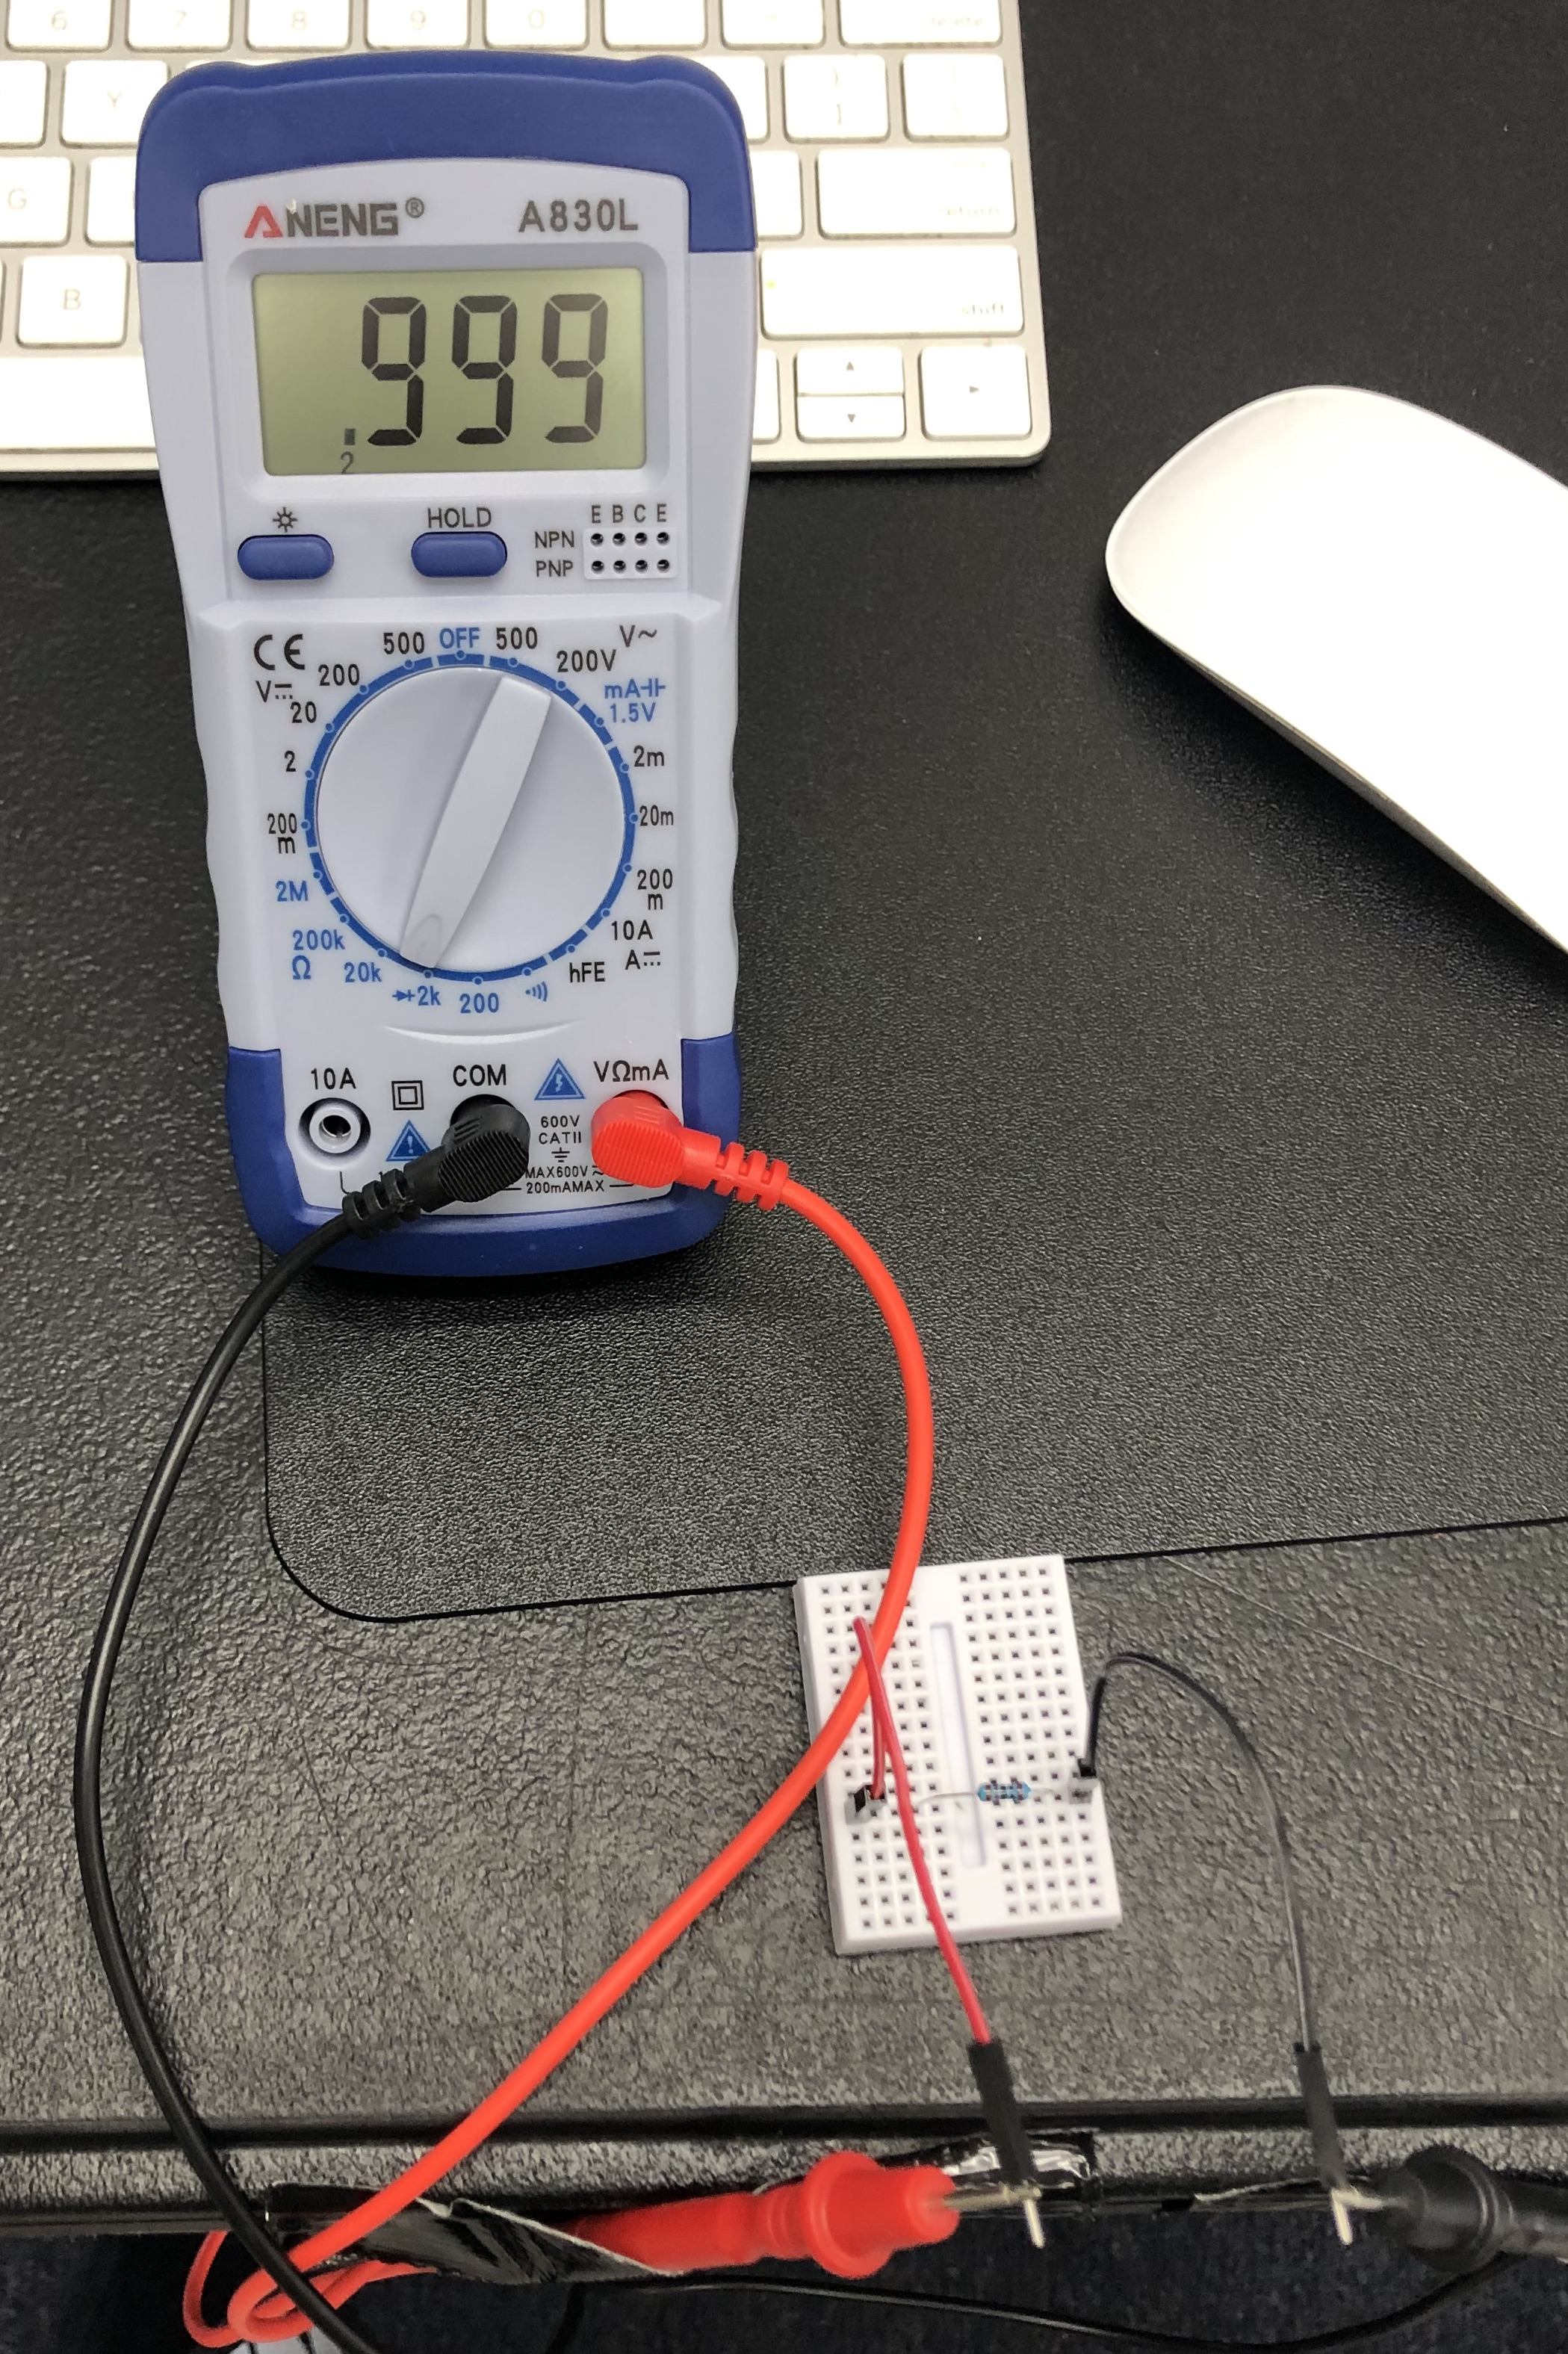
\includegraphics[scale=0.079,height=4.5cm]{R1.jpeg}
    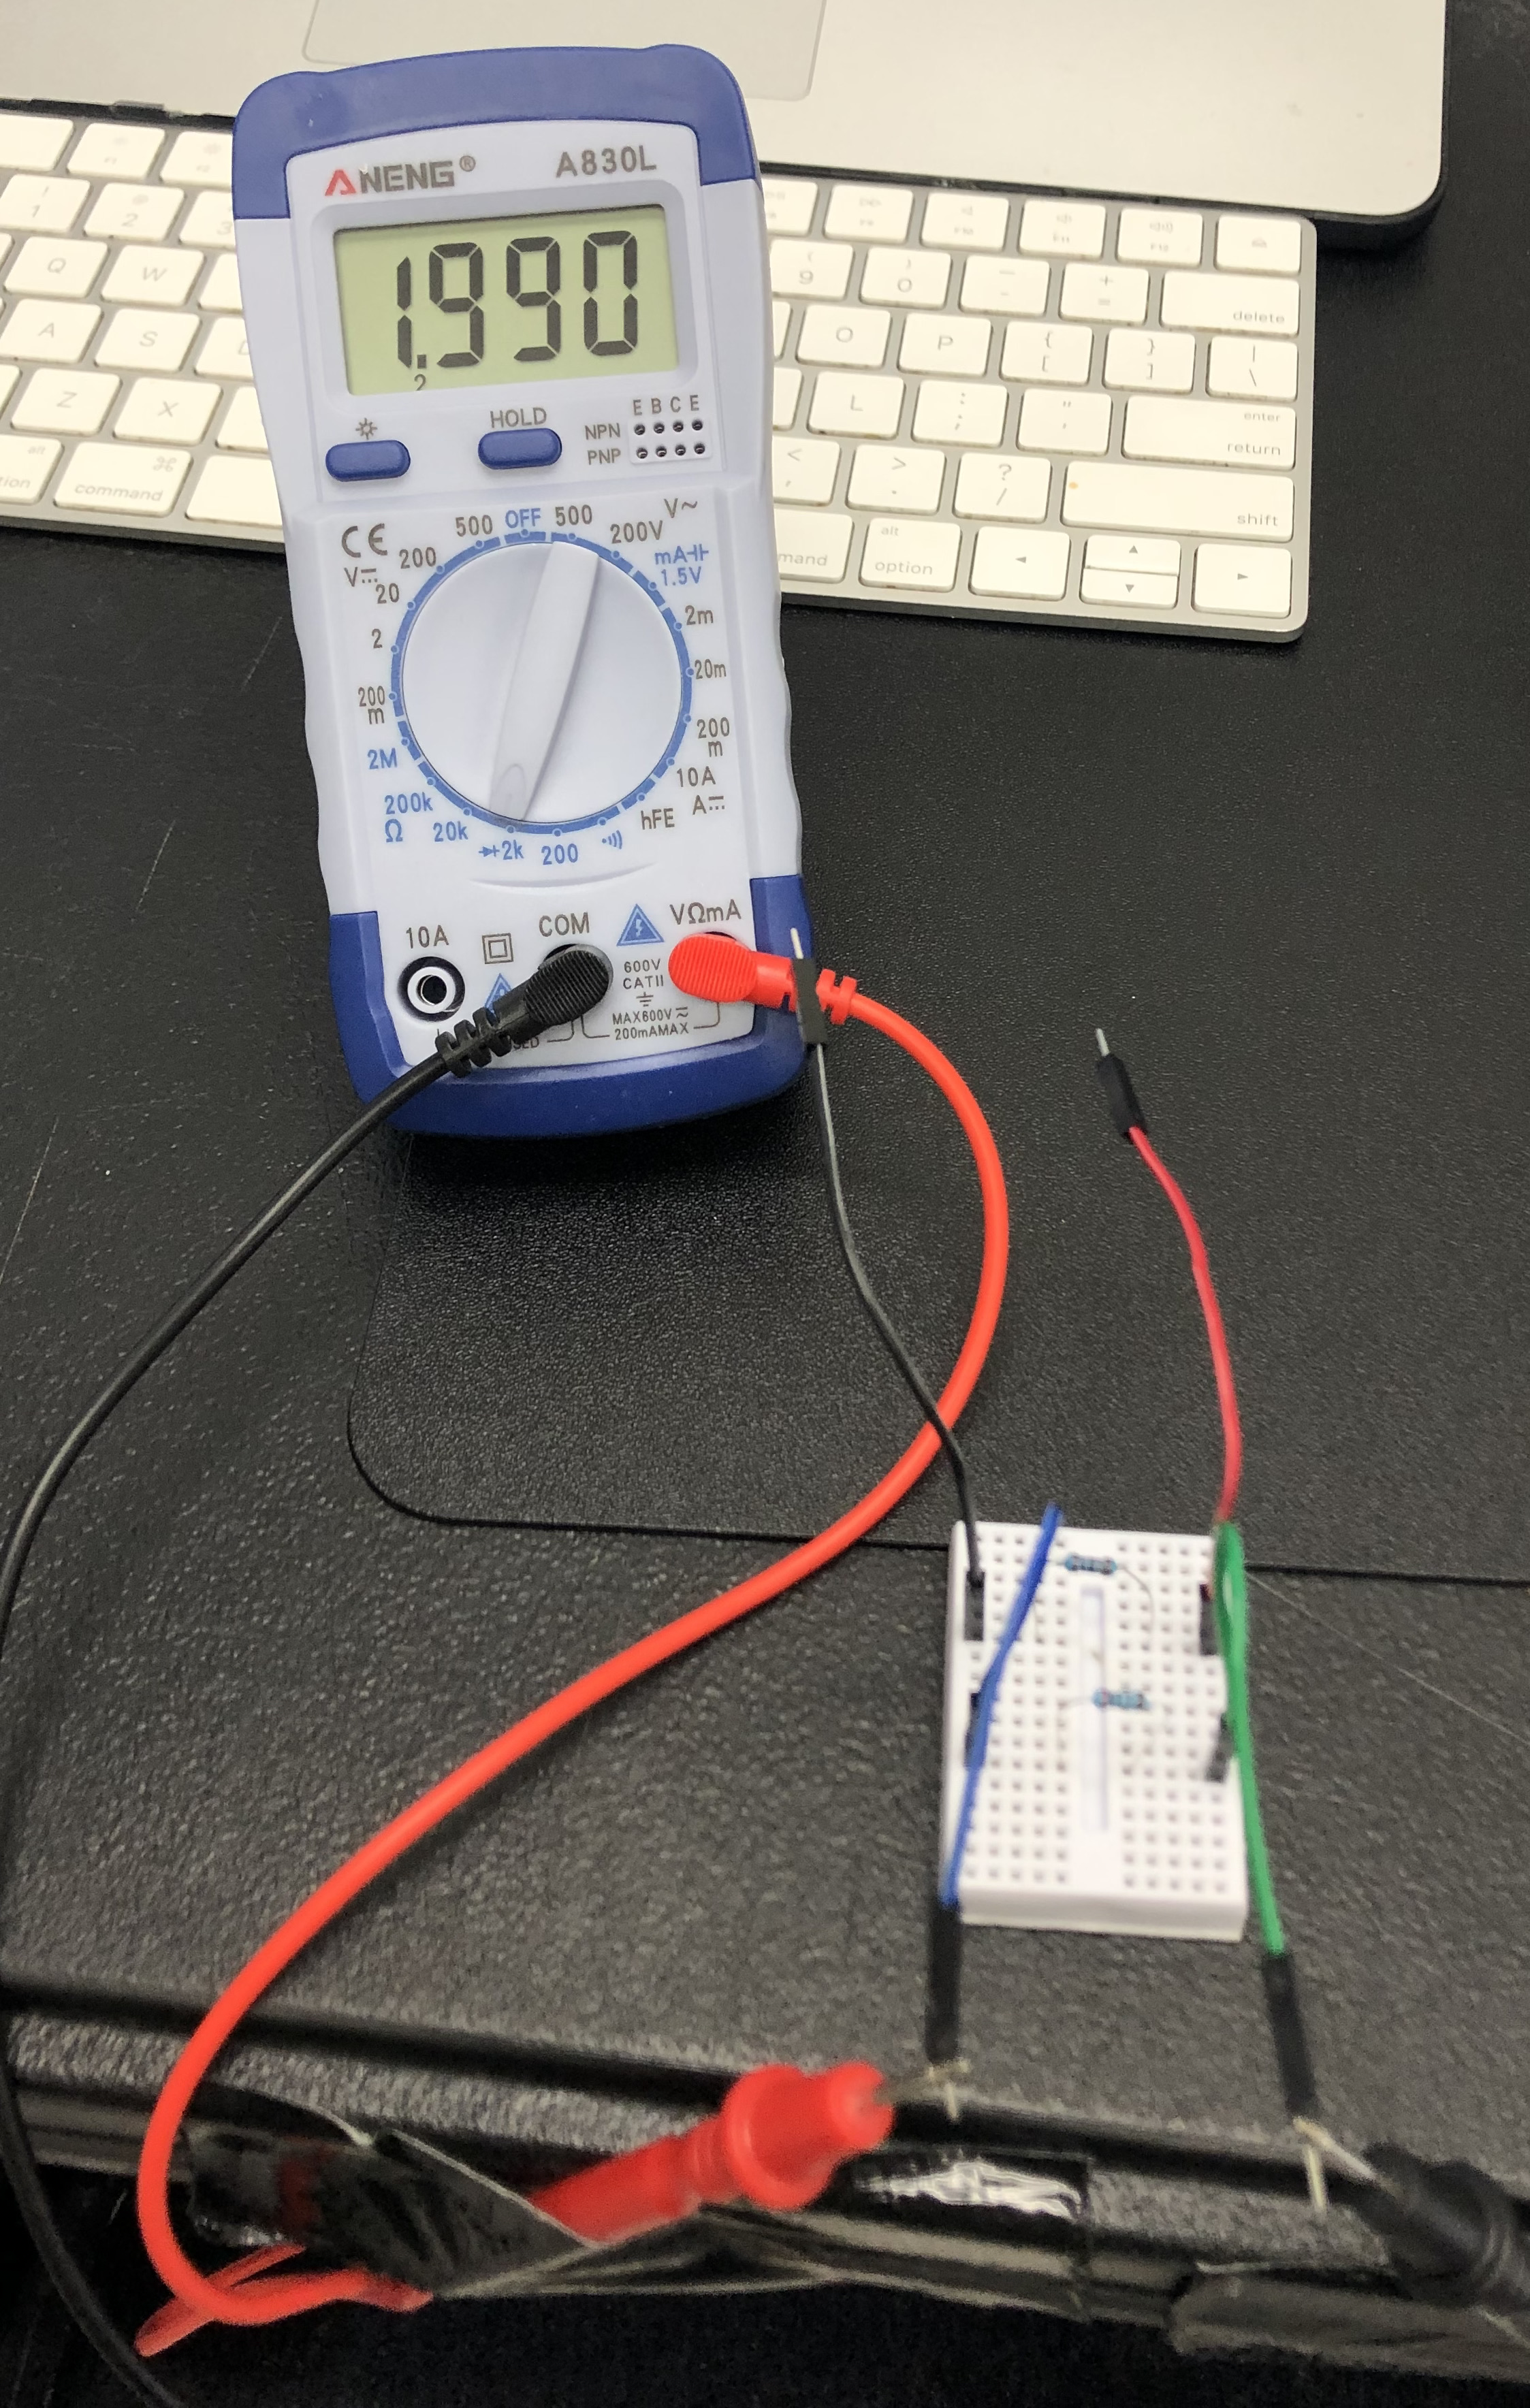
\includegraphics[scale=0.070,height=4.5cm]{R2.jpeg}
    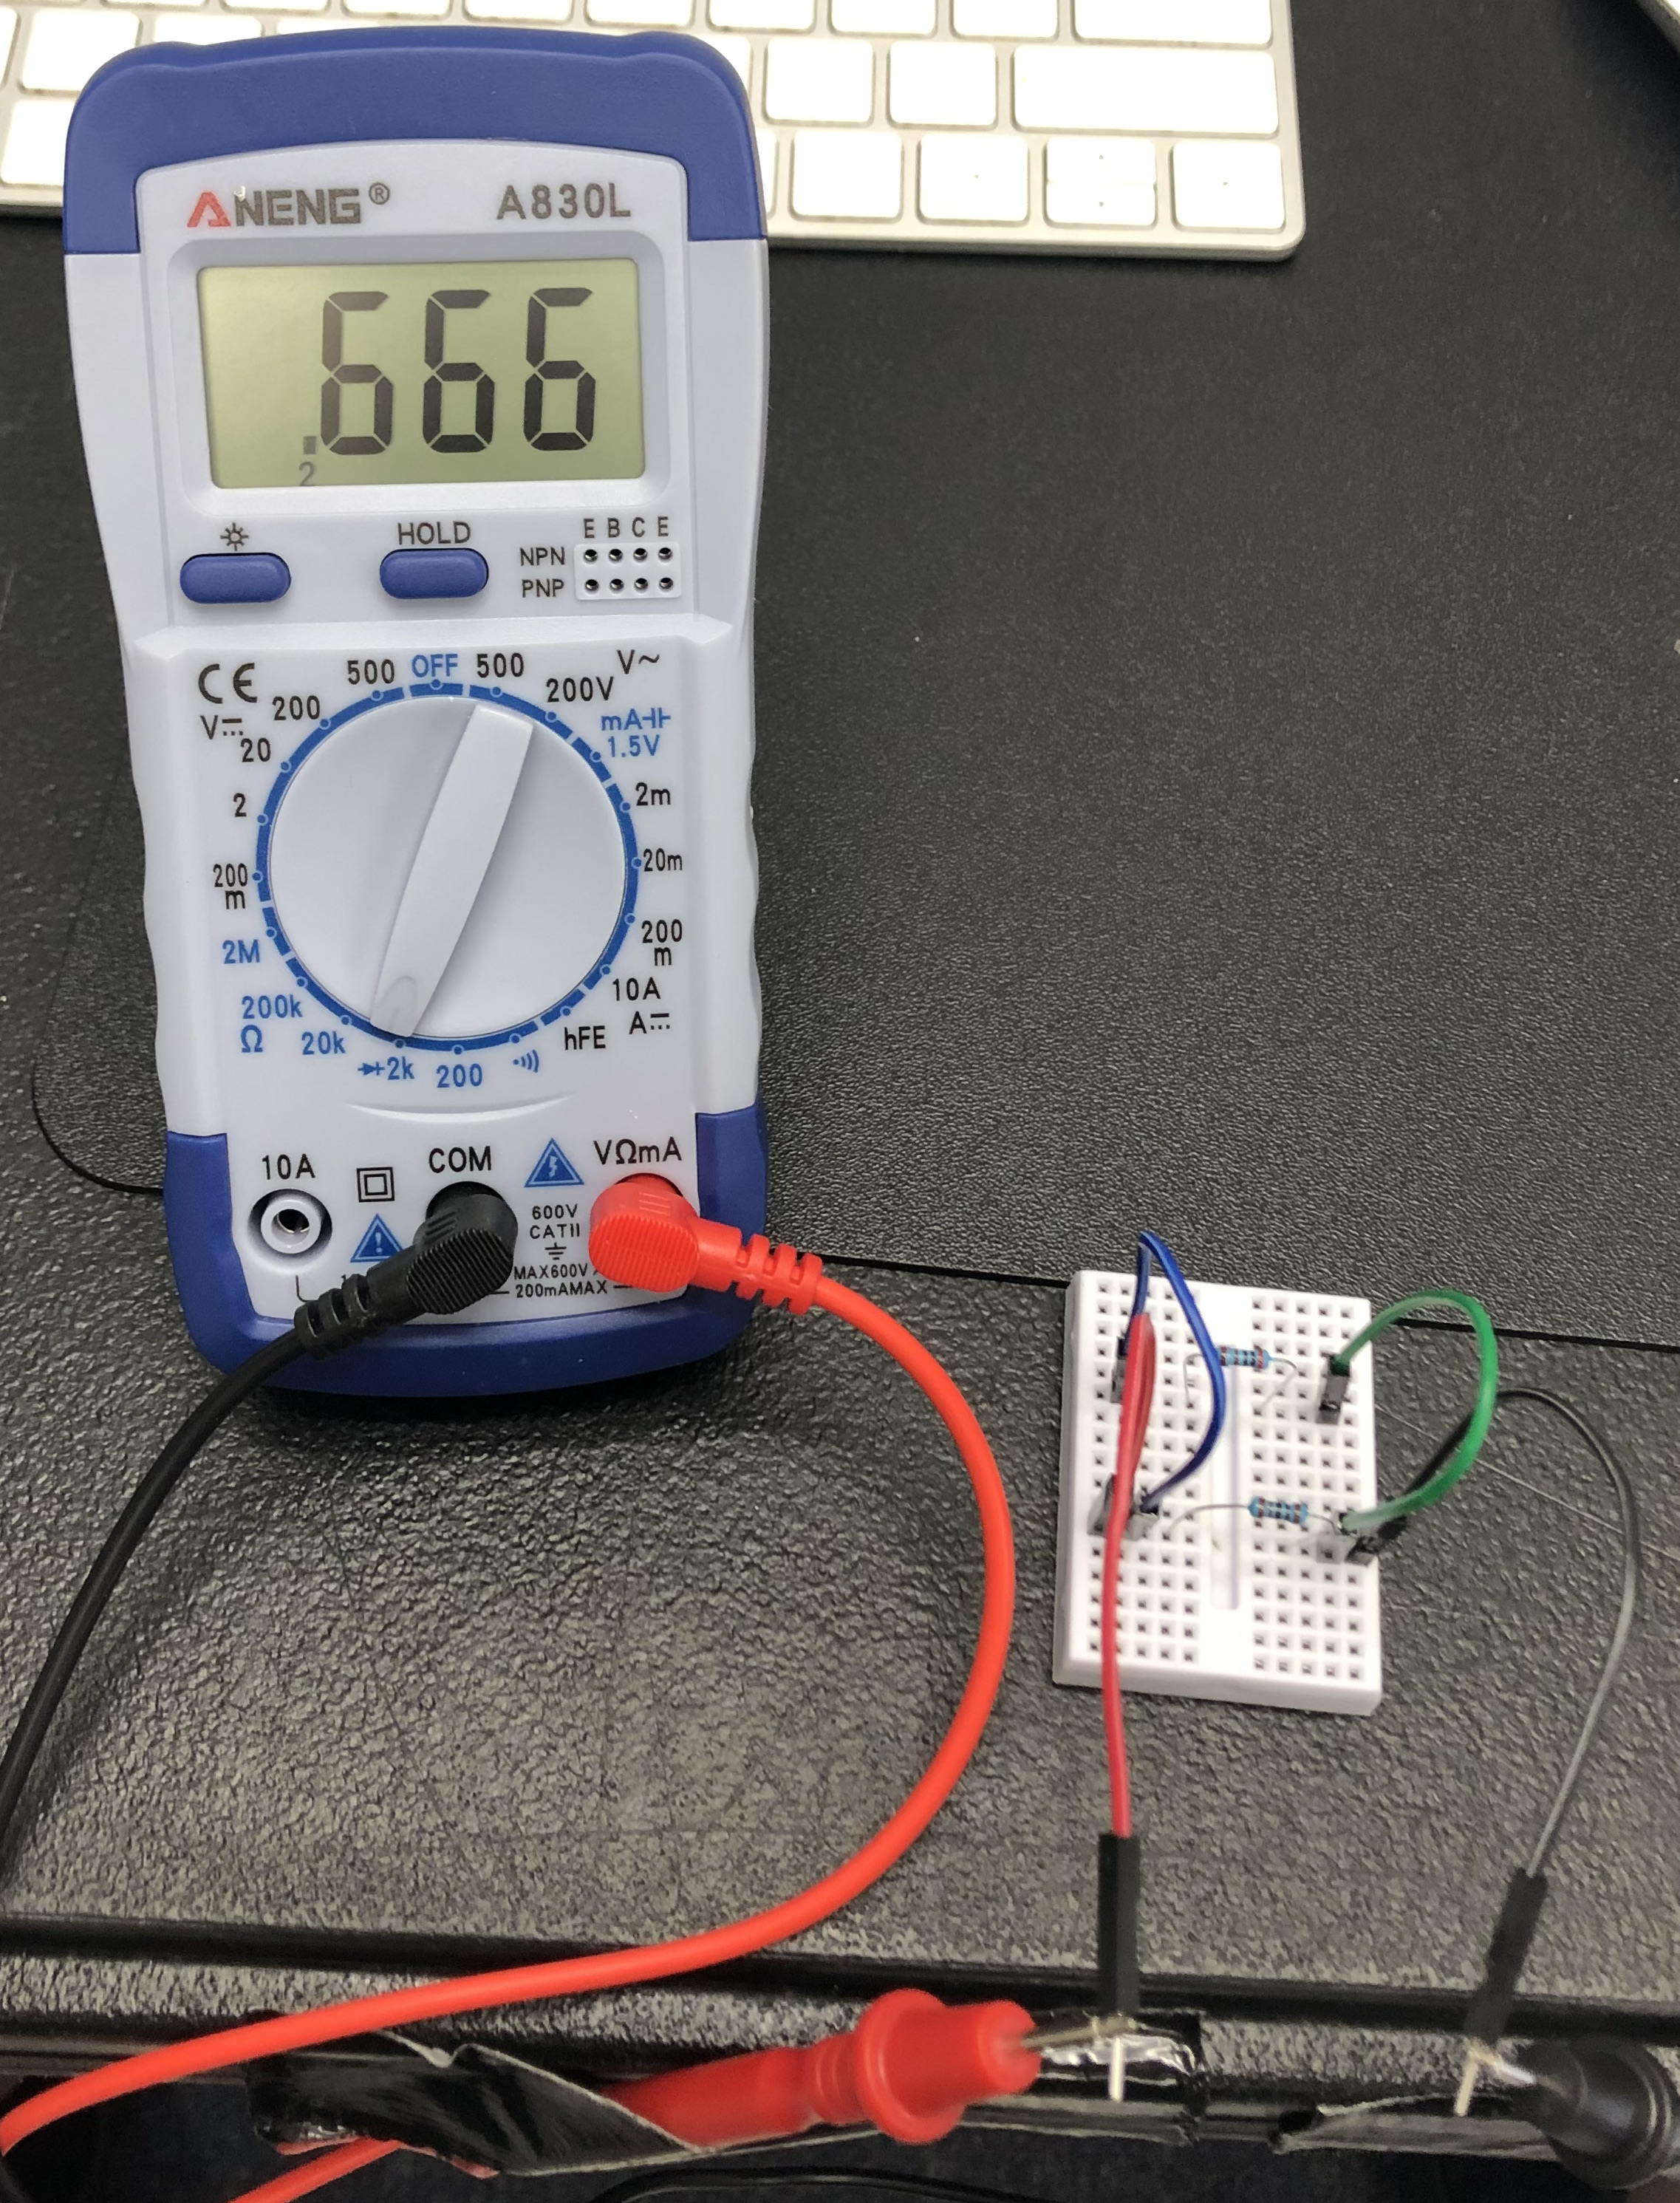
\includegraphics[scale=0.083,height=4.5cm]{RP.jpeg}
    \subsection*{Graph 2}
    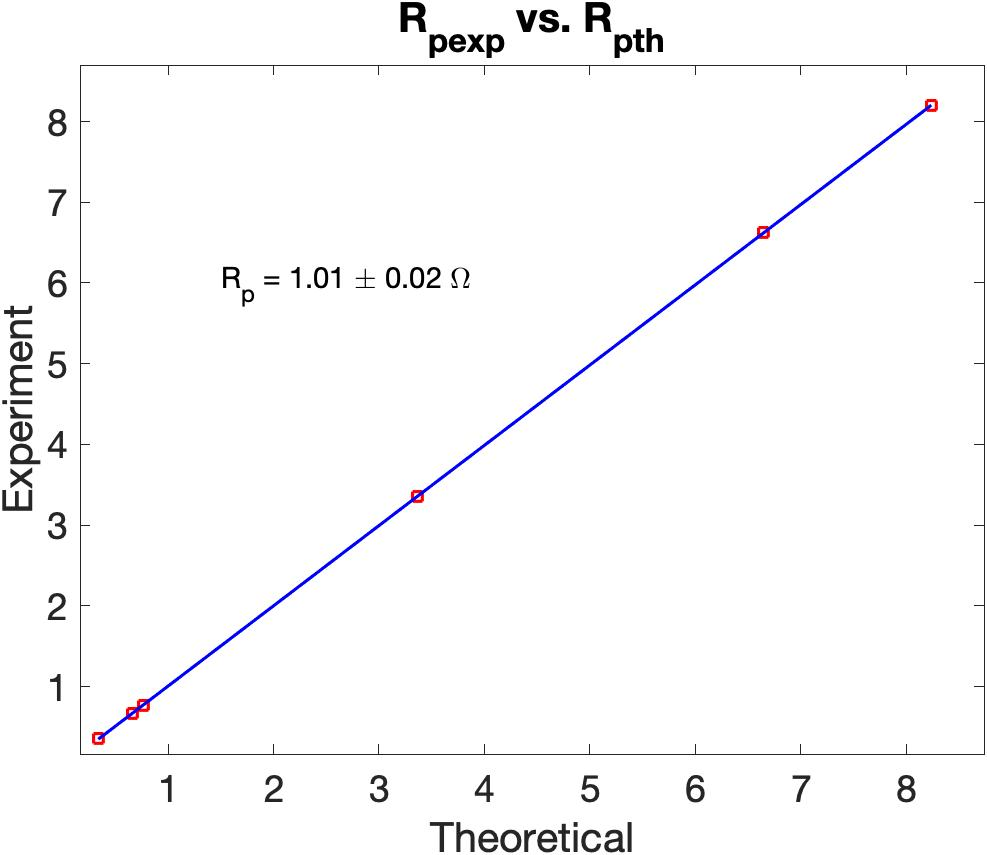
\includegraphics[scale=0.18]{RP_graph.jpeg}
    \subsection*{Discussion 2}
    \begin{enumerate}
      \item Discuss how well the experimental values of the series networks followed the theoretically expected value and quantify that relation.
      \begin{itemize}
        \item
      \end{itemize}
    \end{enumerate}
  \end{center}
\end{table}
\end{document}